\documentclass[a4paper,11pt,twoside,openright]{article}

\usepackage[toc,page]{appendix}
\usepackage{amsmath}
\usepackage{geometry}
\usepackage{graphicx}
\usepackage{subcaption}
\usepackage{multirow}
\usepackage[section]{placeins}
\usepackage{array}
\usepackage[nottoc,numbib]{tocbibind}
%\usepackage{titlesec}

\geometry{margin=1in}
\graphicspath{ {Images/} }

\newcolumntype{?}[1]{!{\vrule width #1}}
\newcommand{\Mod}[1]{\ (\mathrm{mod}\ #1)}

\let\oldsection\section
\def\section{\cleardoublepage\oldsection}

%\setcounter{tocdepth}{4}

%\titleformat{\paragraph}
%{\normalfont\normalsize\bfseries}{\theparagraph}{1em}{}
%\titlespacing*{\paragraph}
%{0pt}{3.25ex plus 1ex minus .2ex}{1.5ex plus .2ex}

\begin{document}

%%%%%%%%%%%%%%%%%%%%%%%%%%%%%%%%%%%%%%%%%%%%%%%%%%%%%%%%%%%%%%%%%%%%%%%%%%%%%%%
% TITLEPAGE                                                                   %
%%%%%%%%%%%%%%%%%%%%%%%%%%%%%%%%%%%%%%%%%%%%%%%%%%%%%%%%%%%%%%%%%%%%%%%%%%%%%%%
\pagenumbering{gobble}
\centering
\vspace*{6cm}
        {\huge Developing AntBot: \par A navigational system inspired by \par the
          insect brain \par}
\vspace{1cm}
{\Large \textit{Robert E. F. Mitchell}}

\vspace{3cm}

{\large Master of Informatics \par}
{\large Informatics \par}
{\large School of Informatics \par}
{\large The University of Edinburgh \par}
\large \today \par

\vfill
Supervised by\par
Dr. Barbara Webb

\newpage
\thispagestyle{empty}
\mbox{}
\newpage

%%%%%%%%%%%%%%%%%%%%%%%%%%%%%%%%%%%%%%%%%%%%%%%%%%%%%%%%%%%%%%%%%%%%%%%%%%%%%%%
% ACKNOWLEDGEMENTS                                                            %
%%%%%%%%%%%%%%%%%%%%%%%%%%%%%%%%%%%%%%%%%%%%%%%%%%%%%%%%%%%%%%%%%%%%%%%%%%%%%%%
\pagenumbering{roman}
\centering
{\LARGE \textbf{Acknowledgements}}
\begin{flushleft}
 {\small \textit{Pending . . .} }
\end{flushleft}  

\newpage
\thispagestyle{empty}
\mbox{}
\newpage

%%%%%%%%%%%%%%%%%%%%%%%%%%%%%%%%%%%%%%%%%%%%%%%%%%%%%%%%%%%%%%%%%%%%%%%%%%%%%%%
% DECLARATION                                                                 %
%%%%%%%%%%%%%%%%%%%%%%%%%%%%%%%%%%%%%%%%%%%%%%%%%%%%%%%%%%%%%%%%%%%%%%%%%%%%%%%
\centering
{\LARGE\textbf{Declaration}}
\begin{flushleft}
  {\small
    I declare that this dissertation was composed by myself, the work
    contained herein is my own except where explicitly stated otherwise
    in the text, and that this work has not been submitted for any other
    degree or professional qualification except as specified.
    \par 

    \textit{Robert Mitchell}}

\end{flushleft}

\newpage
\thispagestyle{empty}
\mbox{}
\newpage

%%%%%%%%%%%%%%%%%%%%%%%%%%%%%%%%%%%%%%%%%%%%%%%%%%%%%%%%%%%%%%%%%%%%%%%%%%%%%%%
% ABSTRACT                                                                    %
%%%%%%%%%%%%%%%%%%%%%%%%%%%%%%%%%%%%%%%%%%%%%%%%%%%%%%%%%%%%%%%%%%%%%%%%%%%%%%%
\centering
{\LARGE\textbf{Abstract}}
\begin{flushleft}
  {\small \textit{Pending . . .}}
\end{flushleft}

\newpage

%%%%%%%%%%%%%%%%%%%%%%%%%%%%%%%%%%%%%%%%%%%%%%%%%%%%%%%%%%%%%%%%%%%%%%%%%%%%%%%
% CONTENTS                                                                    %
%%%%%%%%%%%%%%%%%%%%%%%%%%%%%%%%%%%%%%%%%%%%%%%%%%%%%%%%%%%%%%%%%%%%%%%%%%%%%%%
\tableofcontents
\newpage

%%%%%%%%%%%%%%%%%%%%%%%%%%%%%%%%%%%%%%%%%%%%%%%%%%%%%%%%%%%%%%%%%%%%%%%%%%%%%%%
% FIGURES                                                                     %
%%%%%%%%%%%%%%%%%%%%%%%%%%%%%%%%%%%%%%%%%%%%%%%%%%%%%%%%%%%%%%%%%%%%%%%%%%%%%%%
\listoffigures
\newpage

%%%%%%%%%%%%%%%%%%%%%%%%%%%%%%%%%%%%%%%%%%%%%%%%%%%%%%%%%%%%%%%%%%%%%%%%%%%%%%%
% TABLES                                                                      %
%%%%%%%%%%%%%%%%%%%%%%%%%%%%%%%%%%%%%%%%%%%%%%%%%%%%%%%%%%%%%%%%%%%%%%%%%%%%%%%
\listoftables
\newpage
\thispagestyle{empty}
\mbox{}
\newpage

%%%%%%%%%%%%%%%%%%%%%%%%%%%%%%%%%%%%%%%%%%%%%%%%%%%%%%%%%%%%%%%%%%%%%%%%%%%%%%%
% INTRODUCTION                                                                %
%%%%%%%%%%%%%%%%%%%%%%%%%%%%%%%%%%%%%%%%%%%%%%%%%%%%%%%%%%%%%%%%%%%%%%%%%%%%%%%
\pagenumbering{arabic}

\raggedright
\section{ Introduction }
Navigation is a complex task. Determining a sequence of actions to reach a
known location, based on a combination of sensory inputs requires a lot of
computational power. Desert ants, are capable of performing such a task
over comparitively huge distances with limited, low resolution sensory
information and remarkable efficiency. While the exact method by which
the ants perform this task is still unknown, a reasonably complete navigational
model can be constructed from existing physiologically plausible components,
which may mimic the insect behaviour.
\newline
\par

In this paper we introduce a combined model, the One Ring (OR)\footnote{[DRAFT]
  This is just a little fun, if it's too on-the-nose I'm happy to change it to
  Extended CX or something a little more serious.
} model for insect
navigation. To be clear, there is no (known) physiological basis for such a
model; however, it is biologically plausible, and may provide insight into
the operation of the real insect brain. The OR model combines the tasks of Visual
Navigation, Path Integration, and Collision Avoidance; using, the Mushroom Body
Circuit (MB)\cite{Ardin2016}, the Central Complex model (CX)\cite{Stone2017},
and Optical Flow Collision Avoidance (OFCA)\cite{Mitchell2018} for each task
at a low level, then combining their outputs to get a form of higher visual
processing (similar to the weighted ``base model'' described in \cite{Webb2018}).
The OR model is a modified Central Complex model, named simply to ensure
distinction between the two models. The individual components are all
bioloigically plausible and two of three are known to be physiologically
plausible. \cite{Ardin2016, Stone2017, Mitchell2018}.
\newline
\par

This project primarily extends the work done in \cite{Mitchell2018}. As such we
continue using the AntBot platform; a robot constructed for the express purpose
of experimenting with the algorithms in the \textit{Ant Navigational Toolkit}
\cite{Wehner2009}.

\subsection{ Motivation }
Currently, a full base model for insect navigation does not exist
\cite{Webb2018}. We here aim to take the abstraction presented by \textit{Webb}
and create a biologically plausible implementation using our three-system
approach. Both the MB and CX models have been implemented and tested on AntBot
previously \cite{Scimeca2017, Mitchell2018, Eberding2016, Zhang2017}, and a model
combining the two has also been attempted by \textit{Zhang} in \cite{Zhang2017}.
This is used as an inspiration and will be discussed further in Section
\ref{MBBackground}.
\newline
\par

The previous AntBot implementations have demonstrated good performance of the CX
and MB models individually \cite{Scimeca2017, Mitchell2018}. Performance of
a combined system has also been shown to be reasonable, however, it is less
consistent than we would desire\cite{Zhang2017}. In the combined model from
\cite{Zhang2017} we note two key problems: A fixed outbound route, and fixed
component weightings. We address the former by adding the OFCA component to our
model; as in \cite{Mitchell2018}, the AntBot will follow a non-deterministic
outbound route through a cluttered arena. The latter brings up the more
complicated question of plausible synaptic plasticity which, while undoubtedly
interesting, lies outside the scope of this project. It is worth noting that here
may also have been unknown tecnical issues with the robot which affected results
(see \cite{Mitchell2018}).
\newline
\par

While \cite{Mitchell2018} provides a reasonable collision avoidance system
based on optical flow, it does not fit so neatly into the OR model. We therefore
aim to explore an alternative, yet still biologically plausible collision
avoidance system which will fit into the OR model.
\newline
\par

Our ultimate hope, is to provide some insight into the precise biological
systems in play during a point-to-point navigational task.

\subsection { Practical Goals }
We aim to build upon the experimental scenario from \cite{Mitchell2018}. The
robot will be tested by allowing it to navigate through a cluttered environment
using a collision avoidance system. The navigational systems will then be
tasked with bringing the robot home through the cluttered environment using
a combination of visual information, a path integration vector, and
collision avoidance.
\newline
\par

In order to achieve this experimental goal, we break the project down
into four components:

\begin{enumerate}
\item{The first stage will involve solving some technical issues
  picked up by \cite{Mitchell2018}; making any hardware/software adjustments
  required to provide a solid foundation on which to develop.}

\item{ The second stage
will involve investigating existing systems and establishing experimental
metrics. This stage will involve research and review of new topics (the
main one being the Central Complex model for Path Integration), and their
implementations on the robot (if they exist). This stage will look to establish
appropriate metrics by testing the existing CX model in a non-deterministic
navigational task (see Section \ref{sec:methods}).}

\item{This stage will involve the setup and testing of the individual components
  of the OR model. Building the modified optical flow system, adapting the work
  from \textit{Zhang} to combine the MB model with the CX, and finally, putting
  the three pieces together.}

\item{Finally, the collection and compilation of results from the combined system
and the individual systems.}
\end{enumerate}


\subsection { Results }
This work is based on work done previously by Leonard Eberding, Luca Scimeca,
Zhaoyu Zhang, and Robert Mitchell.
\cite{Eberding2016, Scimeca2017, Zhang2017, Mitchell2018}.
\newline

Significant contributions of this project:
\begin{enumerate}
\item{
  Research and installation of a new compass sensor for the AntBot control
  systems.
}

\item{
  A major code refactor has taken place to make AntBot more usable for this
  project, and make it more accessible for future students.
}

\item{
  Addition of a calibration system to allow the user to auto-detect the position
  of the camera lens attachment (see Section \ref{sec:platform}).
}

\item{
  Results gathered for the Central Complex model using a non-deterministic
  outbound route.
}

\item{
  \textit{[FUTURE]}
  Construction of a modified optical flow collision avoidance system, and a
  modified Mushroom Body model based on \cite{Mitchell2018} and \cite{Zhang2017}
  respectively.
}

\item{
  \textit{[FUTURE]} Construction of a biologically plausible ``base model'' for
  insect navigation. The One Ring (OR) model.
}

\item{
  \textit{[FUTURE]} Results indicating the capability of the OR model.
}
\end{enumerate}
\newpage

%%%%%%%%%%%%%%%%%%%%%%%%%%%%%%%%%%%%%%%%%%%%%%%%%%%%%%%%%%%%%%%%%%%%%%%%%%%%%%%
% BACKGROUND                                                                  %
%%%%%%%%%%%%%%%%%%%%%%%%%%%%%%%%%%%%%%%%%%%%%%%%%%%%%%%%%%%%%%%%%%%%%%%%%%%%%%%
% Brief summaries of OF and MB, more detailed discussion of CX
\section{ Background }
This project builds directly upon \cite{Mitchell2018}. We first provide a review
of the relevant background topics from that paper, before developing the relevant
ideas further for this project. This will be a very brief summary of the work
that took place and any relevant results or new perspectives. For more detail,
please consult \cite{Mitchell2018}.


\subsection{ Optical Flow for Collision Avoidance } \label{OFBackground}
Optical flow is a large and diverse area of study. As such, we will not provide
a complete background on the fundamental principles. Relevant terms will be
explained, however, a succinct background of the concepts necessary for this
paper can be found in \cite{Mitchell2018}. A comprehensive introduction is
given by \textit{O'Donovan} in \cite{ODonovan2005}.
\newline
\par

The main driving point in this paper is the integration of multiple navigational
systems into a single model, namely, the Central Complex.
Optical flow flitering worked well for a standalone collision avoidance system,
however, it does not fit so neatly into the CX model. We therefore require a
different approach. The relevant background revisits the concept of the
\textit{focus of expansion} (FOE) from \cite{Mitchell2018, ODonovan2005}.
The FOE is the point from which all optical flow vectors originate. The location
of the FOE can tell us things about the motion, and depth of the image.
\newline
\par

In \cite{Mitchell2018}, the FOE was used explicitly to compute time-to-contact
with an obstacle. In this work, we instead use it simply to determine the
potential location of an obstacle. As stated in \cite{Burger1989}, computing the
FOE is not trivial. Following \cite{Mitchell2018} we will be using a dense
optic flow field (tracking motion for every pixel in the image) as the
computation of sparse fields was shown to be unreliable on the AntBot. This makes
the problem more difficult; the basic from-flow method for computing the FOE
given by \cite{ODonovan2005} is computationally complex for a dense flow field
\cite{Mitchell2018}. The time taken to compute may become prohibitive. We will
therefore look at a few different methods including that given by
\textit{O'Donovan}.

\subsubsection{The from-flow method}
This is the method given by \textit{O'Donovan} and discussed in
\cite{Mitchell2018}. We term it the \textit{from-flow} method, as we must first
compute an optic flow field, from which we compute the FOE. The FOE is computed
simply as:

\begin{equation}
  \label{eq:foe}
  FOE = (A^TA)^{-1}A^T\mathbf{b}
\end{equation}

\begin{equation*}
  \begin{split}
 A = 
\begin{bmatrix}
  a_{00} & a_{01}\\
  \dots  & \dots \\
  a_{n0} &  a_{n1}
\end{bmatrix}
\qquad
\end{split}
\begin{split}
\mathbf{b} =
\begin{bmatrix}
  b_0 \\
  \dots \\
  b_n
\end{bmatrix}
\end{split}
\end{equation*}
\newline

Where, each pixel $p_i = (x, y)$ has associated flow vector $\mathbf{v} = (u,v)$.
Finally, set $a_{i0} = u$, $a_{i1} = v$ and $b{i} = xv - yu$. Note that this
computation and explanation have been more or less copied from
\cite{Mitchell2018} for the benefit of the reader. For more details, the reader
should consult \cite{ODonovan2005}.
\newline
\par

This method for estimating the focus of expansion was originally given by
\textit{Tistarelli et al.} in their paper
\textit{Dynamic Stereo in Visual Navigation}\cite{Tistarelli1991, ODonovan2005},
and it serves as an excellent example for the reason the FOE is so difficult to
compute. In theory, we should be able to take any two vectors $\mathbf{u}$,
$\mathbf{v}$ from the flow field, and compute the point at which lines
running along them intersect. This point of intersection would give us the
FOE\cite{ODonovan2005}. While wonderfully simple, this method only works for
a perfect flow field. In reality, flow fields are imperfect; for example,
visual noise can cause disruptions to areas of the field. Therefore picking two
arbitrary vectors could lead to an erroneous FOE. Unravelling the matrix notation
of Equation \ref{eq:foe}, shows this to be a least squares technique;
essentially, we try to fit the best FOE to the flow field given.

%\subsubsection{The fuzzy method}
%Instead of attempting to estimate an exact point which is likely to be the
%FOE, \textit{Burger and Bhanu} propose a method for computing a small region
%which is likely to contain the FOE. This region is referred to as the
%\textit{fuzzy FOE}\cite{Burger1989}.
%\newline
%\par

%Their motivation for using a region as opposed to a point is the rotational
%aspect of motion. If we have a wheeled robotwith a fixed camera, the camera has
%(broadly) two aspects to its motion: Translational and Rotational. Translation is
%experienced when the robot moves forward, or backward in a straight line
%(i.e. the camera is moving directly into the image or away from it). Rotation
%occurs when the robot turns. If the robot moves in a straight line, the rotation
%component can be ignored; similarly, if the robot turns on the spot, the
%translation component can be ignored. Many papers on using the FOE will ignore
%rotation. In many applications (including our own) this is completely acceptable;
%for example, if the robot only ever moves in straight lines with stationary
%turns. Their discussion takes place in the context of an Autonomous Land Vehicle
%(ALV) which is capable of arcing movements, so both components come into play.
%\newline
%\par

%Perhaps counter-intuitively, their computation still requires testing and
%working with a single FOE.

%The computation takes two steps:
%\begin{enumerate}
%\item{
%  Search for a location (they call it $\mathbf{x}_{min}$) of local minimum error
%  starting from an arbitrary location $\mathbf{x}_0$.
%}

%\item{
%  \textit{Grow} a connected region around this $\mathbf{x}_{min}$ until some
%  criterion is met.
%}

%\end{enumerate}

%The criterion they choose is an accumulated error volume threshold; i.e. setting
%a limit on the amount of error that can be contained in the fuzzy FOE;
%intuitively, the smaller the error, the more likely the region is to contain the
%FOE.

%\subsubsection{The direct method}

\subsection{ The Mushroom Body for Visual Navigation } \label{MBBackground}
The Mushroom Body model is an artificial neural network which models
the mushroom body structures present in the insect brain\cite{Ardin2016}. It
consists of three layers: Projection Neurons (PNs), Kenyon Cells (KCs) and
Mushroom Body Output Neurons (MBONs). These MBONs are also referred to as
Extrinsic Neurons (ENs) by older works, we use MBON herein. The original MB model
proposed by \textit{Ardin et al.} for navigation in \cite{Ardin2016} contained
360 visual PNs (vPNs), 20,000 KCs, and a single MBON. Every KC connects to the
MBON, and each KC also connects to 10 vPNs chosen uniform randomly. The KC-MBON
connections all start with weight $w=1$. The figure and caption from
\textit{Ardin et al.} is given here in Figure \ref{fig:mb}.

\begin{figure}
  \centering
  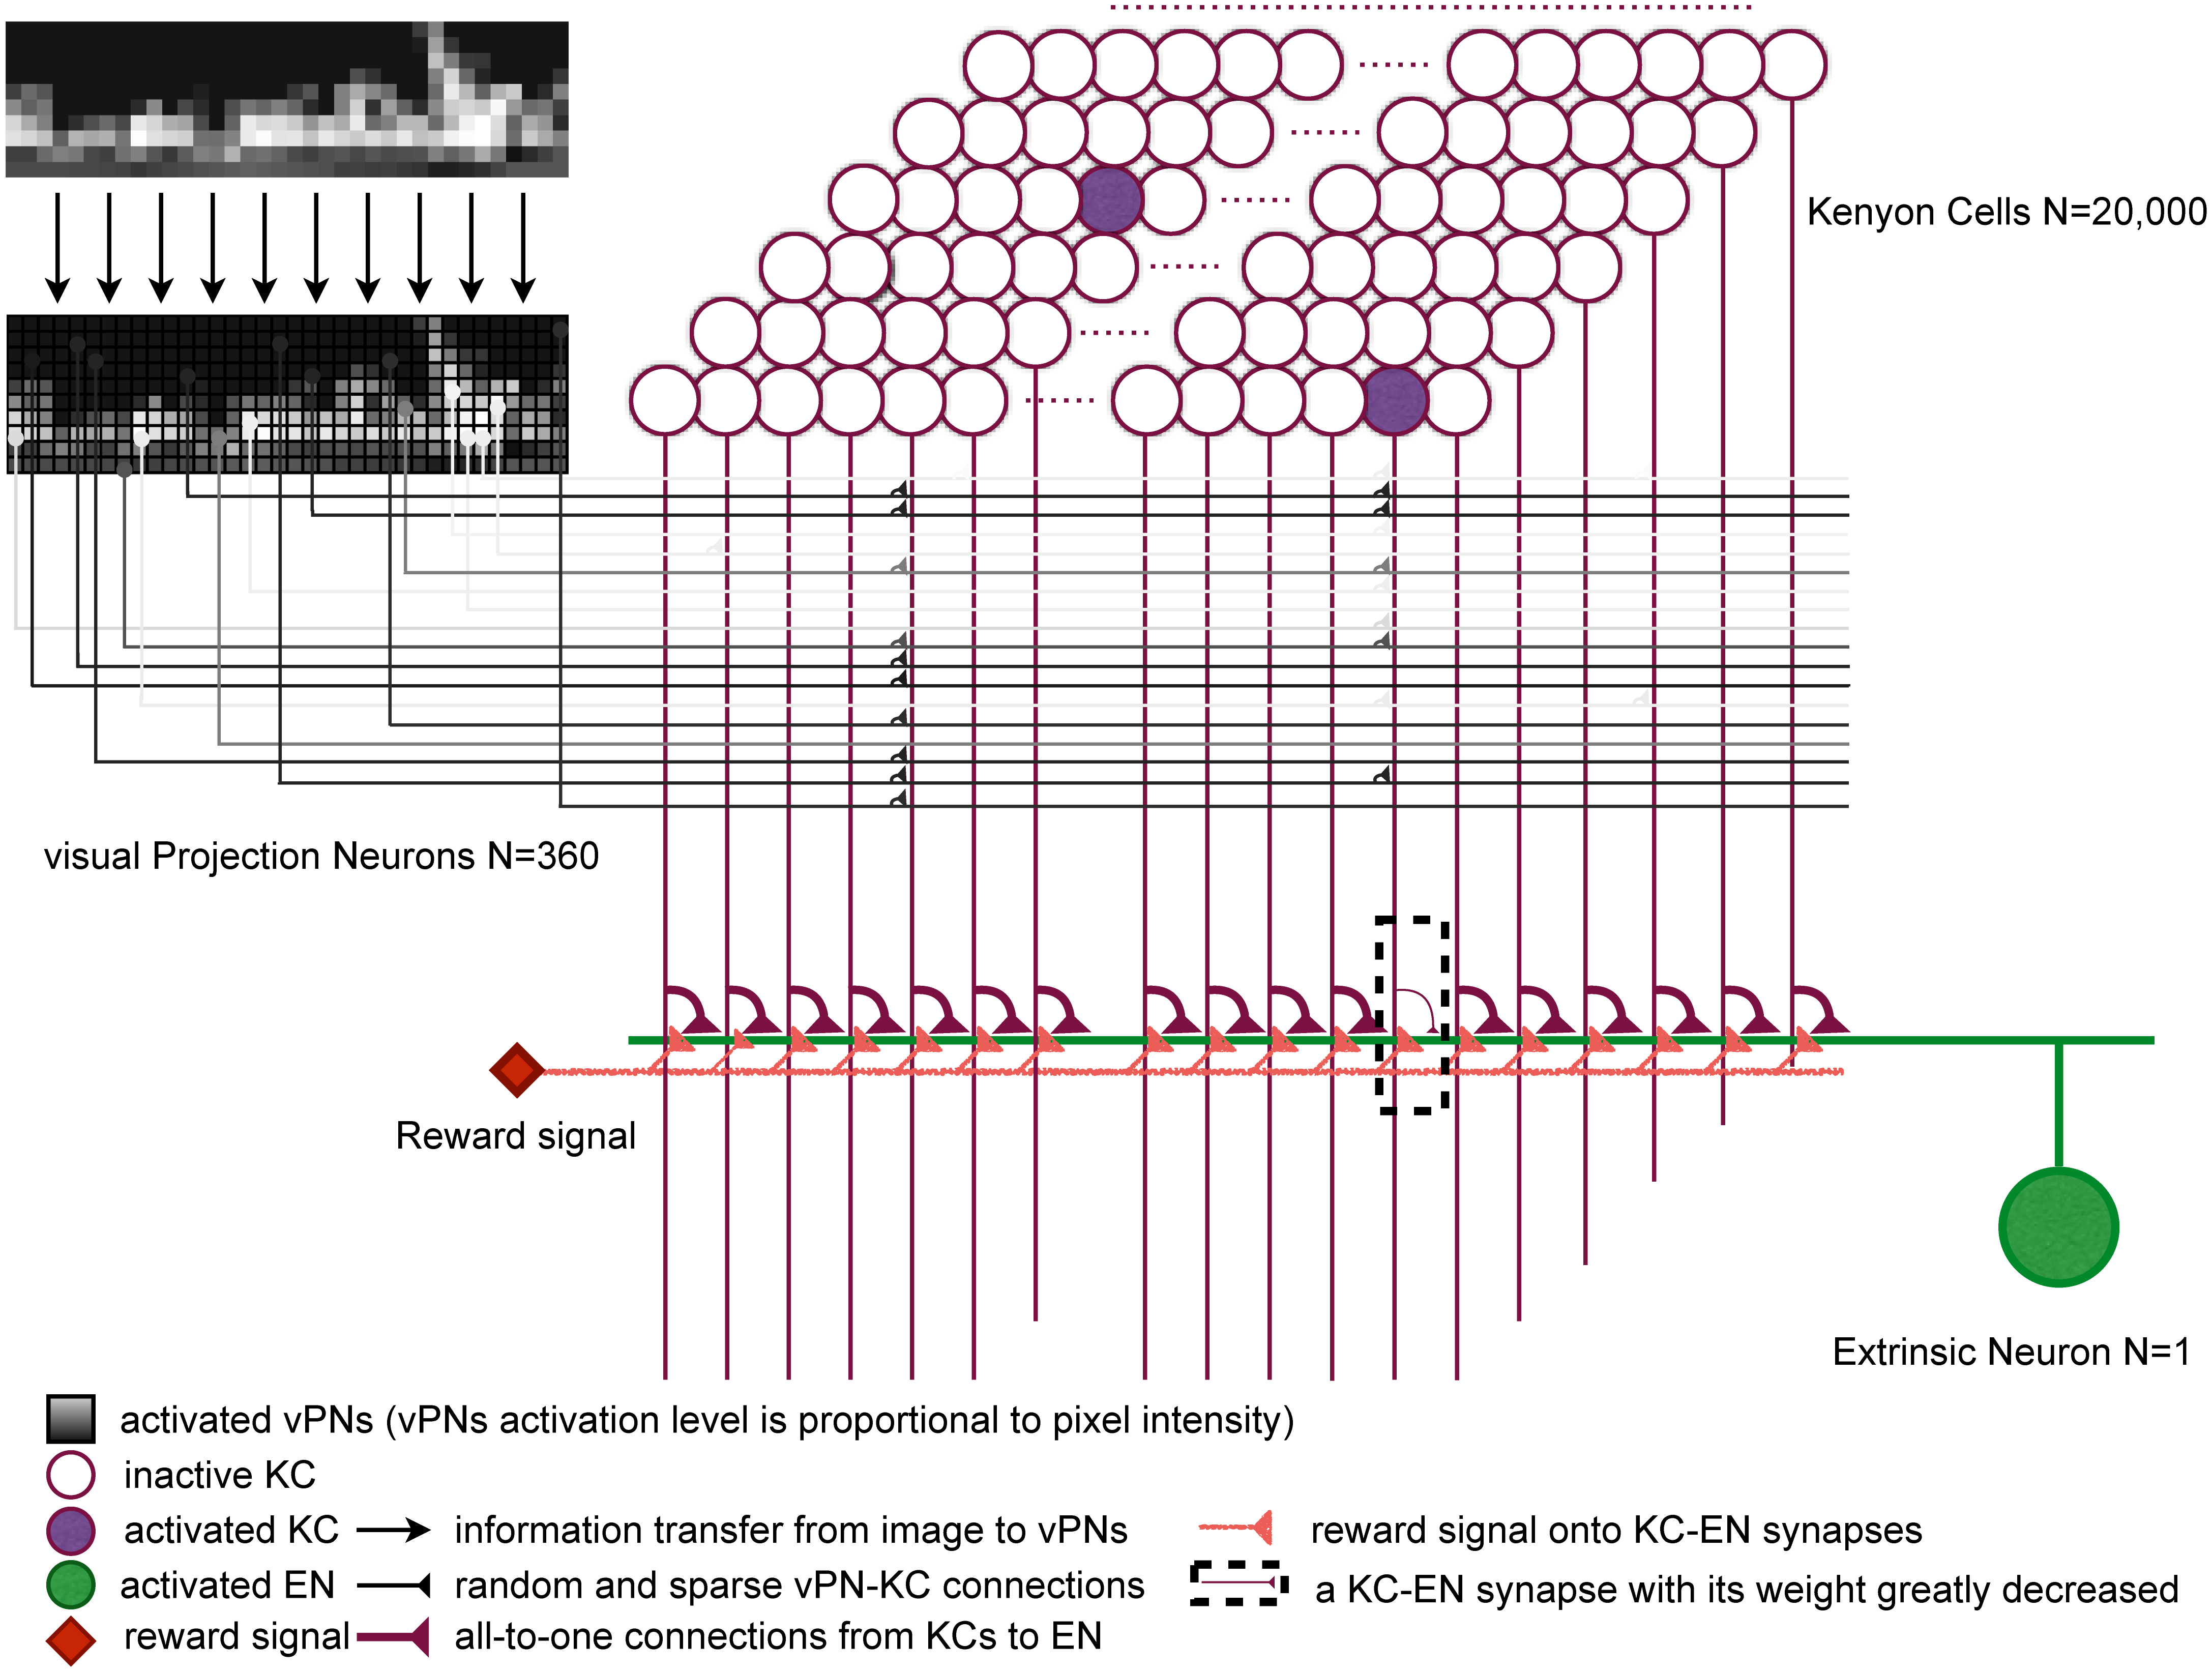
\includegraphics[width=0.7\textwidth]{Ardin2010MBModel}
  \caption{\label{fig:mb} The Mushroom Body circuit: (Caption from
    \textit{Ardin et al.}, Figure 2; note, their description and figure uses
    ``EN'' instead of ``MBON''): Images (see Fig 1) activate the visual
    projection neurons (vPNs). Each Kenyon cell (KC) receives input from 10
    (random) vPNs and exceeds firing threshold only for coincident activation
    from several vPNs, thus images are encoded as a sparse pattern of KC
    activation. All KCs converge on a single extrinsic neuron (EN) and if
    activation coincides with a reward signal, the connection strength is
    decreased. After training the EN output to previously rewarded (familiar)
    images is few or no spikes.}
\end{figure}

In the implementation by \textit{Ardin et al.}
and previous AntBot implementations, captured images were converted to greyscale
and downsampled\cite{Ardin2016, Eberding2016, Zhang2017, Mitchell2018}. As such,
each pixel can be described by a brightness (greyscale value). Each KC has
a brightness threshold. Learning occurs by showing patterns (images) to the vPNs.
KCs each have a brightness activation threshold; each KC sums the brightness of
all connected vPNs and compares that sum to the threshold. If the total
brightness is greater than the threshold then the KC is \textit{activated} and
the weight of the KC-MBON connection is lowered from 1 to 0. Thus, each image
shown to the vPNs should induce a sparse activation pattern in the KC layer.
\newline
\par

To determine image familiarity during the recapitulation process, a pattern is
projected onto the vPNs (again giving a sparse pattern of KC activation.
The MBON then sums the weights of all active KCs to obtain a familiarity measure;
the lower the MBON output, the more familiar the image. Different route following
strategies have been implemented (scanning\cite{Ardin2016, Eberding2016,
  Zhang2017}, Klinokinesis\cite{Zhang2017}, combination with the CX
model\cite{Zhang2017}(see below), and visual scanning\cite{Mitchell2018}); but, most
commonly, some form of scanning is used whereby the agent scans an arc for the
most familiar direction.
\newline
\par

This has been a brief explanation for context. Part 1 gives slightly deeper
insight\cite{Mitchell2018} (particularly in relation to AntBot projects), and of
course the work \textit{Ardin et al.} can give the full details\cite{Ardin2016}
\newline
\par

The MB model described above has been tested on the AntBot in three different
works (albeit using different methods and metrics); the network as presented in
\cite{Eberding2016, Zhang2017, Mitchell2018} differs only in the number of PNs
present (900 vPNs are used in all three works). More relevant to this work, is
the proposed modification given by \textit{Zhang}, whereby, 8 MBONs are present
as opposed to 1 (see Section \ref{CXMBBackground}).
\newline
\par

\subsection{ The Central Complex for Path Integration } \label{CXBackground}
The Central Complex (CX) is a highly conserved structure present in the insect
brain\cite{Pfeiffer2014, Stone2017}. Though the finer structural details and
component position may vary, the basic composition is more or less the same
across species \cite{Pfeiffer2014}. Organization and function of the
various parts of the CX are given by \textit{Pfeiffer and Homberg} in
\cite{Pfeiffer2014}\footnote{[DRAFT] I would like to include a short overview
  of the neurobiology but have left it until I can properly read through
  \cite{Pfeiffer2014}. I think I will need to leave this out, however, as I'm
  not sure where to stop in terms of detail given by
  \textit{Pfeiffer and Hormberg}; also I may run out of time!
}
\newline
\par

We instead direct our attention to the CX model presented by
\textit{Stone et al.} which is the first neural model for path integration
in the insect brain, with structure drawn purely from physiology. Interestingly,
this model is actually an advancement of an earlier model presented by
\textit{Haferlach et al.}, which was \textit{evolved} using a Genetic Algorithm
(GA). We present this also, purely for the sake of interest.

\subsubsection{The Central Complex Model}
The Central Complex model is a six layer artificial neural network presented by
\textit{Stone et al.} which has been shown to provide a plausible neural
substrate for Path Integration (PI) both in simulation and on the AntBot platform
\cite{Scimeca2017, Stone2017}. The model presented is shown in Figure
\ref{fig:cx}. Splitting the model into its six layers, we get a breakdown of
functionality:
\newline
\par

\begin{itemize}
\item{Layer 1: Heading preprocessing (TL), Speed (TN)}
\item{Layer 2: Heading preprocessing (CL1)}
\item{Layer 3: Heading (TB1)}
\item{Layer 4: Memory (CPU4)}
\item{Layer 5: Normalisation and Inhibition (Pontine Neurons)}
\item{Layer 6: Steering/output (CPU1)}
\end{itemize}

\begin{figure}[h!]
  \centering
  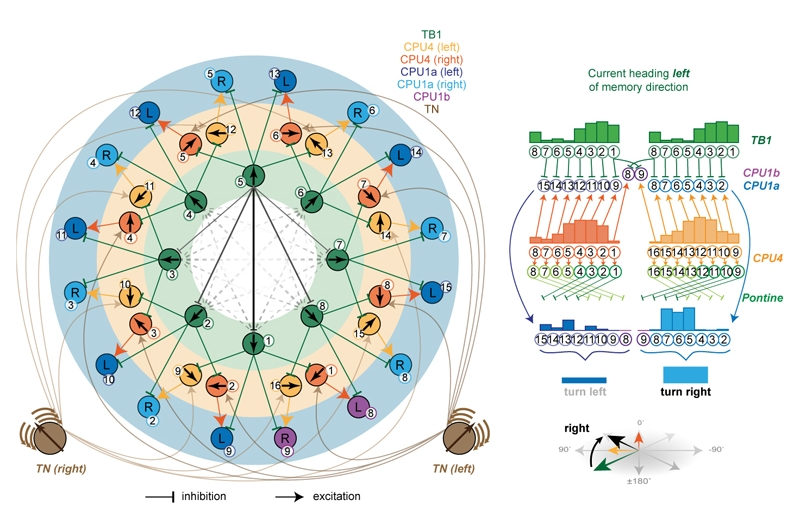
\includegraphics[width=\textwidth]{StoneCXModel}
  \caption{\label{fig:cx} The Central Complex model presented by
    \textit{Stone et al.}. (Left) This graph demonstrates the basic structure of
    the CX model (Figure 5G from \cite{Stone2017}). Pontine neurons have been
    excluded for clarity.
    (Right) This graph shows how signals propogate through the network where the
    current heading lies to the left of the desired heading, i.e. a right turn
    should be generated (Figure 5I from \cite{Stone2017}). The numbers given at
    each layer on the right correspond to the numbers given for each neuron
    in the graph on the left.
  }
\end{figure}

Figure \ref{fig:cx} shows four types of neuron: TN (Tangential Neuron), TB1
(green), CPU4 (yellow and orange), and CPU1 (dark blue, light blue, and purple).
\newline
\par

While Figure \ref{fig:cx} (Left) shows a distinction between CPU1a (blue) and
CPU1b (purple) neurons, we will ignore this distinction; for clarity, the
physiological mapping between these CPU1 subtypes in the Upper Central Body (CBU)
and the Protocerebral Bridge (PB) is different, but the function they serve in
the Central Complex is the same \cite{Stone2017}; thus, the distinction makes
no difference in the model. Similarly the normalisation and inhibition function
of the Pontine Neurons only has an effect when the agent experiences holonomic
motion (motion where the view direction does not match the direction of travel);
as AntBot is incapable of such motion, we can safely ignore the function of
the Pontine Neurons also; in our case, the Pontine Neurons would have the
same activity patterns as the CPU4 neurons \cite{Stone2017}. Figure \ref{fig:cx}
(Right) shows how the Pontine inhibition is structured.
\newline
\par

\begin{figure}[h!]
  \centering
  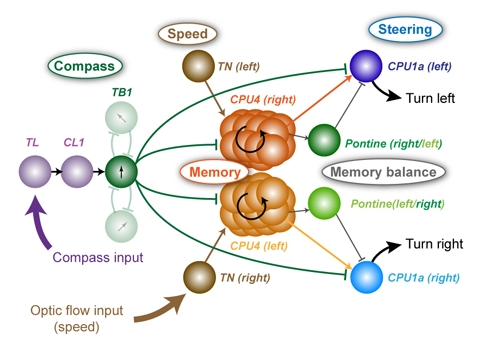
\includegraphics[width=0.7\textwidth]{Figure5F}
  \caption{
    \label{fig:cxlayer} Here we can see the layers of the CX model and
    how they fit together. A heading signal is input to the TL neurons,
    propogating through the CL layer to TB1 (heading ring-attractor) and
    CPU4 (memory). TN neurons (speed sensitivity) input directly to CPU4.
    So, the combination of heading and speed inputs to CPU4 gives a measure
    of distance travelled in a particular direction; this facilitates generation
    of a steering command in CPU1 providing a mechanism for Path Integration.
  }
\end{figure}

We now break down the different neuronal types and their proposed functions.
Citation is given, but for the avoidance of any doubt, the following descriptions
are adapted from \textit{Stone et al.} (see STAR Methods) \cite{Stone2017}.

\textbf{Simulated Neurons:}
Each neuron is described by its firing rate, where the firing rate $r$ is
a sigmoid function of the input $I$:

\begin{equation}
r = \frac{1}{1 + e^{-(aI - b)}}
\end{equation}

where $a$ and $b$ are parameters which control the slope and offset of the
sigmoid function \cite{Stone2017}. Optionally, Gaussian noise may be added
to the output. The input to each neuron is a weighted sum of the activity
of each neuron that synapses onto it; say neuron $j$, the input is:

\begin{equation}
  I_j = \sum_{i} w_{ij} \cdot r_i
\end{equation}

The weights used by \textit{Stone et al.} can only be 0, 1, or -1 for
no-connection, excitatory, or inhibitory respectively \cite{Stone2017}.

% Function of CL & TL
\textbf{TL \& CL1:}
The TL neurons are the input point for heading information. In the ant brain
this heading information comes from a \textit{sky-compass}; the ant eye contains
cells sensitive to polarized light which allows the ant to infer an accurate,
allothetic direction from vision. Interestingly, there is also evidence that ants
have the capability to infer a direction without a view of celestial cues,
suggesting they may have access to some other signal, the candidate signal being
the geomagnetic field \cite{Fleischmann2018, Grob2017}. The TL neurons have been
shown to be polarisation sensiive across multiple insect species \cite{Stone2017}
(see STAR Methods). Each TL neuron has a preferred direction (i.e. a specific
direction of poliarisation sensitivity) $\theta_{TL}$, and there are 16 such
neurons representing the 8 directions around the agent (i.e.
$\theta_{TL} \in \{ 0^{\circ}, 45^{\circ}, 90^{\circ}, 135^{circ}, 180^{\circ},
225^{\circ}, 270^{\circ}, 315^{\circ}\} $) \cite{Stone2017}. Together, the 16
TL neurons encode the heading of the agent in a single timestep; each neuron
receives input activation as:

\begin{equation}
  I_{TL} = cos( \theta_{TL} - \theta_{h} )
\end{equation}

where $\theta_{TL}$ is the preferred heading of the neuron as above, and
$\theta_{h}$ is the current heading of the agent. In the next heading layer,
there are 16 CL1 neurons which use inhibition to invert the polarisation
response \cite{Stone2017}. \textit{Stone et al.} comment that these neurons
effectively make no difference to the model and are included for completeness.
They are also included in previous AntBot projects which make use of the CX model
\cite{Zhang2017, Scimeca2017}. On AntBot, the heading is derived from the onboard
compass on the mobile phone (see Section \ref{sec:platform}).
\newline
\par

% Function of TN
\textbf{TN:}
There are 4 TN neurons which act as an input for speed information. The TN
neurons are sensitive to optical flow, and can be split into two subtypes:
TN1, and TN2. \textit{Stone et al.} showed that TN1 neurons are inhibited by
simulated forward flight and excited by simulated backward flight, while TN2
neurons are inhibited by simulated backward flight and excited by simulated
forward flight \cite{Stone2017}. Each of the four TN neurons has a tuning
preference; these tuning preferences were measured in bees as approximately
$+45^{\circ}$/$-45^{\circ}$ for TN2, and $+135^{\circ}$/$-135^{\circ}$ for TN1
(where $0^{\circ}$ is straight ahead). In short, we have TN$1_{left}$,
TN1$_{right}$, TN$2_{left}$, and TN$2_{right}$. It is thought that these neurons
provide a (or part of a) mechanism for odometry by allowing the model to
integrate speed with respect to time giving a distance measure \cite{Stone2017}.
\textit{Stone et al.} give the speed calculation from the TN neurons
as:

\begin{equation}
  I_{TN_{L}} =
  [ sin(\theta_{h} + \phi_{TN}) \quad cos(\theta_{h} + \phi_{TN}) ]\mathbf{v}
\end{equation}

\begin{equation}
  I_{TN_{R}} =
  [ sin(\theta_{h} - \phi_{TN}) \quad cos(\theta_{h} - \phi_{TN}) ]\mathbf{v}
\end{equation}

where $\mathbf{v}$ is the velocity of the agent in Cartesian coordinates,
$\theta_h \in [0^{\circ}, 360^{\circ})$ is the current heading of the agent, and
$\phi_{TN}$ is the preferred angle of that TN neuron \cite{Stone2017}.
\newline
\par

% Function of TB1
\textbf{TB1:}
There are eight TB1 neurons, each with a directional preference $\theta_{TB1}$,
which correspond to the eight cardinal directions in the model. Each TB1 neuron
receives excitatory input from the pair of CL1 neurons that have the same
directional preference. The TB1 layer contains inhibitory connections between
peer neurons where each TB1 neuron strongly inhibits other TB1 neurons with
opposite directional preferences (see Figure \ref{fig:cx}) forming a
\textit{ring attractor}\cite{Stone2017}. The weighting for an arbitrary
inhibitory connection from neuron $i$ to neuron $j$ is given by:

\begin{equation}
  w_{ij} =
  \frac{cos(\theta_{TB1,i} - \theta_{TB1,j}) - 1}{2}
\end{equation}

where $\theta_{TB1,i}$ is the direction preference of TB1 neuron $i$ (similarly
for $\theta_{TB1,j}$). The total input for each TB1 neuron from the CL1 layer
at timestep $t$ is:

\begin{equation}
  I_{TB1_{j}^{(t)}} =
  (1 - c) \cdot r_{CL1_j}^{(t)} + c \cdot \sum_{i = 1}^{8} w_{ij}
  \cdot r_{CL1_j}^{(t - 1)}
\end{equation}

where $c = 0.33$ is a scaling factor which determines the relative strength
of excitation from the CL1 layer and inhibition from other TB1 neurons. This
network layer produces a stable heading encoding which provides accurate
input for the CPU4 layer, underpinning accurate path integration.
\newline
\par
% Function of CPU4
\textbf{CPU4:}
The 16 CPU4 neurons receive input in the form of an accumulation of
heading $\theta_h^{(t)}$ of the agent, along with a modulated speed response
from the TN2 neurons \cite{Stone2017}. The CPU4 neurons accumulate distance with
direction. The input the CPU4 neurons is given by:

\begin{equation}
I_{CPU4}^{(t)} = I_{CPU4}^{(t - 1)} + h \cdot (r_{TN2}^{(t)} - r_{TN2}^{(t)} - k)
\end{equation}

where $h = 0.0025$ determines the rate of memory accumulation, and $k = 0.1$ is
a uniform rate of memory decay \cite{Stone2017}. All memory cells are initialised
to $I_{CPU4}^{(0)} = 0.5$ and are clipped at each timestep to fall between 0 and
1 \cite{Stone2017}. As shown in Figure \ref{fig:cx}, each TB1 provides input to
two CPU4 neuron, each of which receives input from the TN2 cell in the opposite
hemisphere. As these neurons accumulate distance with respect to a direction,
they provide a population encoding of the \textit{home vector} (the integrated
path back to the nest) \cite{Stone2017}. Interestingly, \textit{Zhang} showed
that the network can be initialised to an arbitrary state, allowing the agent
to navigate along arbitrary vectors \cite{Zhang2017}. While this seems intuitive,
the experimental evidence is valuable and demonstrates that the CPU4 layer could
form a basis for the \textit{vector memory} discussed by \textit{Webb} in
\cite{Webb2018} (see Section \ref{CXMBBackground}).

\textbf{Pontine:}
The pontine neurons project contralaterally connecting opposite CBU columns
(shown in Figure \ref{fig:cx} (Right)). The 16 pontine neurons each receive input
from one CPU4 column \cite{Stone2017}; pontine input can be given simply as:

\begin{equation}
  I_{Pontine}^{(t)} = r_{CPU4}^{(t)}
\end{equation}

% Function of CPU1
\textbf{CPU1:}
There are 16 CPU1 neurons present in the model. Each of which
receives inhibitory input (weight $= -1$) from a TB1 neuron; where, each
TB1 neuron provides inhibitory input to two CPU1 neurons (in the same pattern
as the TB1-CPU4 connections - see Figure \ref{fig:cx}). Each CPU4 neuron also
provides input to a CPU1 neuron (so we get input from vector memory and current
heading). The CPU1 input can be expressed as:

\begin{equation}
  I_{CPU1}^{(t)} = r_{CPU1}^{(t)} + r_{Pontine}^{(t)} - r_{TB1}^{(t)}
\end{equation}

As can be seen the CPU1 neurons also receive input from the pontine neurons.
The CPU1 neurons form two sets, those connecting to left motor units and those
connecting to the right. We choose a direction simply by summing the CPU1 outputs
on both sides and the difference indicates the direction and angle of the
required heading correction:

\begin{equation}
  \theta_h^{(t)} = \theta_h^{(t - 1)} +
  m \cdot (\sum_{i = 1}^{8} r_{CPU1R_{i}} - \sum_{i = 1}^{8} r_{CPU1L_{i}})
\end{equation}

where $m = 0.5$ is a constant \cite{Stone2017}. This effectively describes
how the network generates some turning signal from its current state and inputs
to perform path integration. For further details, please consult \cite{Stone2017}
(the STAR Methods section describes how the model operates).

% STOP POINT: Present model by stone et al. then present the old GA model


\subsection{ The Eight MBON Model (CXMB) } \label{CXMBBackground}
In \cite{Zhang2017}, the MB network is modified by adding 7 MBONs. Each MBON has
its own KC-MBON connection array, each with their own unique weights. Each
connection array corresponds to one of the eight cardinal directions represented
by the TB1 layer of the CX model (namely, $0^{\circ}$, $45^{\circ}$, $90^{\circ}$,
$135^{\circ}$, $180^{\circ}$ ,$225^{\circ}$, $270^{\circ}$, $315^{\circ}$) (see
Section \ref{CXBackground}).
\newline
\par

Image memory now has an associated direction, so, training is performed with
respect to orientation. For example, if the agent has a heading of $45^{\circ}$
when a image is stored, then only the corresponding connection array has its
weights updated during learning. Practically, this is done by querying the TB1
layer of the CX model to find the current direction according to the model
(rather than directly querying the robot's onboard compass). This process is
visualised in Figure \ref{fig:eightmbon}.
\newline
\par

\begin{figure}[h!]
  \centering
  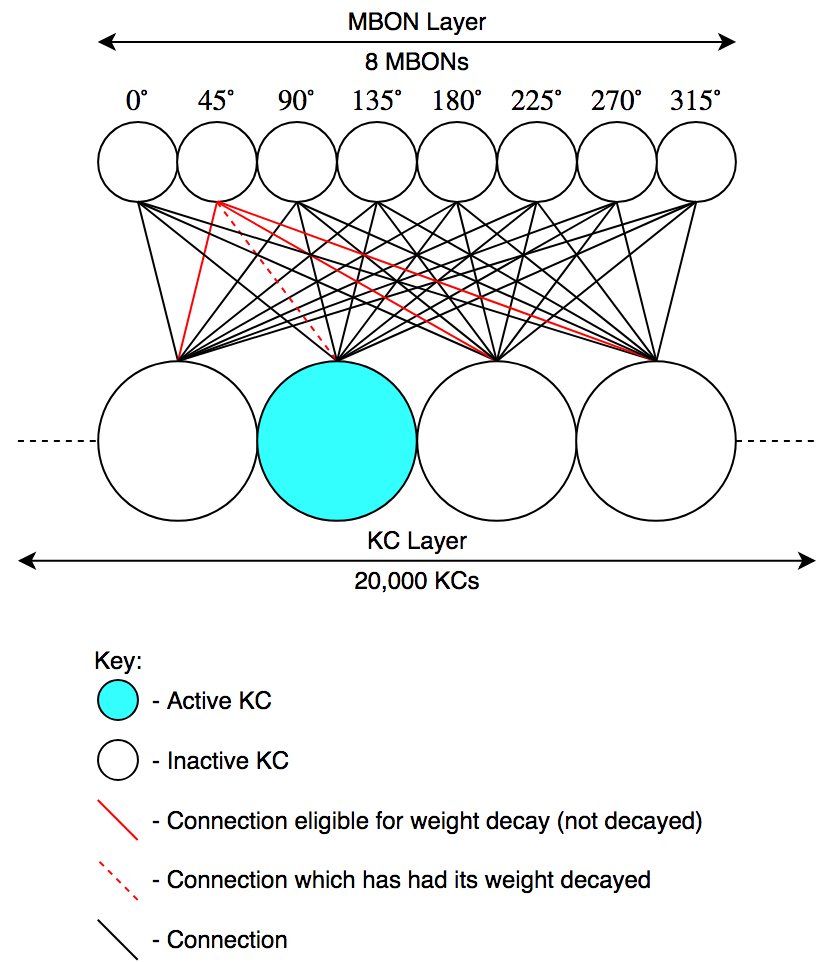
\includegraphics[width=0.9\textwidth]{EightENModel}
  \caption{\label{fig:eightmbon} Our interpretation of the eight MBON model
    proposed by \textit{Zhang}. Every KC connects to every MBON. All connection
    weights start out at $w=1$. Following the example presented in the text,
    if an image being learned corresponds to facing a direction of $45^{\circ}$,
    then only the conncetions to that MBON (highlighted in red) are eligible to
    have their weights modified. Recall, however, that these weights will only
    be modified if the KC was activated (not shown in the figure).
    }
\end{figure}

While, in theory, this eight MBON model could function independently,
\textit{Zhang} uses it to (rather neatly) augment the CX model; this allows
navigation to be performed using a combination of visual memory and path
integration information. The navigation process can be described by a sequence
of equations. We modify the notation slightly for clarity, but the
equations are the same as presented in \cite{Zhang2017}.
\newline
\par

The MB circuit is shown an image in the usual way; however, we now
get eight responses, giving us a response distribution. This distribution can
be interpreted as giving us the most likely direction of travel, when the image
presented was first observed. This distribution requires some modification to
integrate it into the CX response. Let $M_i$ be the familiarity response of the
$i$th MBON; the responses are normalised as:

\begin{equation}
  \bar{M}_i = \frac{M_i}{\Sigma^{8}_{k = 0} M_k}
\end{equation}

Which gives us the normalised response $\bar{M}_i$ between 0 and 1. $\bar{M}_i$
must be inverted so that the most likely direction has the greatest response
(in the MB model, the most familiar direction would give the lowest response):

\begin{equation}
  \bar{M}^{-1}_i = 1 - \bar{M}_i
\end{equation}

This visual response is then combined with the memory response from the CPU4
layer of the CX model to give output at the CPU1 layer:

\begin{equation}
  CPU1_{output} = k \cdot W_{CPU4} \cdot CPU4 + (1 - k) \cdot W_{MBON} \cdot
  \bar{M}^{-1}
\end{equation}

where $k$ is a weighting factor that determines the relative stregths of the CX
response and the MB response in the output ($k = 0.8$ in \cite{Zhang2017}),
$\bar{M}^{-1}$ is the collection of all inverse normalised MBON responses,
$W_{CPU4}$ is a custom matrix\footnote{This is the term used by \textit{Zhang} to
  describe   the $W_{CPU4}$ matrix. More specifically, this matrix describes the
  connections between the CPU4 and CPU1 layers of the CX model.}, $W_{MBON}$ is
an identity matrix that will expand the MBON response array from 8x1 to 16x1
\cite{Zhang2017}.
\newline
\par

In oreder to test the CXMB model, \textit{Zhang} first demonstrated the
functionality of a \textit{copied memory model}. The test of the copied memory
model aimed to prove that the CPU4 state of the agent could be copied and stored,
the CPU4 state modified, and then restored from the copy to allow the agent to
navigate home. The copied memory model was tested by sending the agent on a
pre-determined oubound route to a feeder (chosen at random, but consistent
between trials), copying the CPU4 state, and allowing the robot to navigate home
using the CX model; the CPU4 state will be modified by this homeward navigation.
The agent is then replaced at the feeder, its CPU4 state restored from the copy,
and tasked with navigating home a second time. The copied memory model was tested
as a pre-requisite for testing the CXMB model, however, it demonstrates an
important capability of the CX model; namely, the capability to directly load a
state into its memory in order to navigate; a concept referred to as
\textit{vector memory} in \cite{Webb2018}. Indeed, this concept of vector memory
is shown to be quite a useful tool in insect navigation\cite{Webb2018}.
\newline
\par

The CXMB model is then tested in the same way. The agent follows its oubound
route to the feeder, navigates back once using the CX model (the MB model is
trained on this first inbound trip), is replaced at the
feeder, and finally, tasked with navigating back again, this time using the CXMB
model. To be clear, the CPU4 state of the CX model is stored after the outbound
route, and loaded back into the network before the second inbound trip.
\textit{Zhang} reports that the second inbound trip (using both CXMB) showed
more heading adjustments during its traversal, and, on average, performed
slightly better than a pure CX implementation\cite{Zhang2017}. It should also
be noted that the average performance of both models in \textit{Zhang's} work
was good\cite{Zhang2017}.

\subsection{ Review of Part 1 }
The work in \cite{Mitchell2018} specifically covers the Mushroom Body
and Optical Flow Collision Avoidance. The Mushroom Body model used in
\cite{Mitchell2018} is the same as that used by \textit{Ardin et al.} in
\cite{Ardin2016} though with 900 vPNs as opposed to 360. The model tested
in \cite{Mitchell2018} used a single MBON with a scan-based route following
strategy. The scanning differed from previous works as it was implemented
as an image manipulation algorithm (termed \textit{visual scanning}) instead
of a physical turn performed by the AntBot.
\newline
\par

Multiple OFCA systems were tested, however, in final experiments an
optical flow filtering system is used. In short, a pattern of expected motion is
created, then the actual observed motion is projected on top of it. An absolute
difference is computed between the two and this can tell us if part of the image
is moving faster than we expect. This can be used to detect obstacles. This
strategy proved simple, but effective. While we move away from it for the
bulk of this project, it was used for initial tests of the CX model, as it
provided a simple out-of-the-box method to generate a non-deterministic
path for the model to integrate.
\newline
\par

Both systems functioned well and provided a solid baseline from which we will
work in this project. The MB model proved very capable at following routes
learned in a non-deterministic fashion through a cluttered environment.

\newpage

%%%%%%%%%%%%%%%%%%%%%%%%%%%%%%%%%%%%%%%%%%%%%%%%%%%%%%%%%%%%%%%%%%%%%%%%%%%%%%%
% PLATFORM                                                                    %
%%%%%%%%%%%%%%%%%%%%%%%%%%%%%%%%%%%%%%%%%%%%%%%%%%%%%%%%%%%%%%%%%%%%%%%%%%%%%%%
% High level description of the platform. This section can be short. Refer back
% to Part 1 for detail.
\section{ Platform } \label{sec:platform}
\subsection{ Hardware }
\subsection{ Software }
\subsubsection{ Android } \label{subsubsec:droid}
\subsubsection{ Arduino }
\subsection{ Modifications }
\newpage

%%%%%%%%%%%%%%%%%%%%%%%%%%%%%%%%%%%%%%%%%%%%%%%%%%%%%%%%%%%%%%%%%%%%%%%%%%%%%%%
% METHODS                                                                     %
%%%%%%%%%%%%%%%%%%%%%%%%%%%%%%%%%%%%%%%%%%%%%%%%%%%%%%%%%%%%%%%%%%%%%%%%%%%%%%%
\section{ Methods } \label{sec:methods}
\textit{
  Methods not final, these are included as a rough plan/guide.
  }
\subsection{ Optical Flow }
% Discuss new method (eight directional FOEs)
\subsection{ Visual Navigation }
% Discuss directional recognition, as opposed to scanning.
\subsection{ Path Integration }
% Discuss CX implementation
\subsection{ The Complete System}

\section{Experimentation}\label{sec:test}
\textit{
  Experimentation methods not final, anything in this section illustrates a
  rough plan only.
}
\subsection{General}
\subsection{Collision Avoidance}
% Write new collision avoidance system, test it independently
\subsection{Visual Navigation}
% Do the same for the MB
\subsection{Path Integration}
% And for PI
\newpage

\section{ Results and Evaluation } \label{sec:results}
\textit{Included for skeleton purposes.}
\newpage

\section{ Discussion }
\textit{Included for skeleton purposes.}
\newpage

\bibliographystyle{plain}
\bibliography{working}
\end{document}

